\documentclass[10pt,a4paper]{article}
\usepackage[slovak]{babel}
\usepackage[utf8]{inputenc}
\usepackage{amsmath}
\usepackage{amsfonts}
\usepackage{amssymb}
\usepackage[unicode]{hyperref}
\usepackage{graphicx}

\textwidth 6.5in
\oddsidemargin 0.0in
\evensidemargin 0.0in

\title{Poznámky z počítačových sietí - matroš na štátnice}
\date{15.06.2012}
\author{Peter Csiba, petherz@gmail.com, \url{https://bitbucket.org/petrzlen/fmfi_poznamky}} 

\begin{document}
\maketitle
\tableofcontents

\clearpage

%%%%%%%%%%%%%%%%%%%%%%%%%%%%%%%%%%%%%%%%%%%%%%%%%%%%%%%%%%%%%%%%%%%%%%%%%%%%%%%%
\paragraph{Úvod.}   

Text sú poznámky k oficiálnym \href{štátnicovým otázkam}{http://new.dcs.fmph.uniba.sk/index.php/Studium/Bakalarske/StatneSkusky} a boli spísané počas učenia sa na ne.
Poznámky sa nesnažia ísť do hĺbky (na to je Tanenbaum, Wikipédia a RFC), naopak, snažia sa priniesť intuitívnu predstavu o technológiách a dávať jednotlivé pojmy do súvisu. 
Autor neabsolvoval prednášky ani test z predmetu Počítačové siete. Pán RNDr. Jaroslav Janáček PhD. ohodnotil znalosti počítačových autora pred písaním na D+\footnote{
Čo ho motivuje naučiť sa to poriadne. 
}, takže autor preto neručí za korektnosť textu.
Poznamenajme, že autor sa snažil písať pravdu a len pravdu, keďže jeho odpoveď na štátniciach vychádza z tototo materiálu. V skratke, čitateľ informácie z tohoto textu vstrebáva na vlastné riziko :).

%%%%%%%%%%%%%%%%%%%%%%%%%%%%%%%%%%%%%%%%%%%%%%%%%%%%%%%%%%%%%%%%%%%%%%%%%%%%%%%%
\section{Telekomunikácie}           
%%%%%%%%%%%%%%%%%%%%%%%%%%%%%%%%%%%%%%%
\subsection{Koncept prenosu informácií} 
???

%%%%%%%%%%%%%%%%%%%%%%%%%%%%%%%%%%%%%%%
\subsection{Integrácia}
???
               
%%%%%%%%%%%%%%%%%%%%%%%%%%%%%%%%%%%%%%%
\subsection{MPLS (Multiprotocol Label Switiching)}
Medzi 2. a 3. vrstvou OSI ("layer 2.5" protocol). 
Podporuje priame spojenia, aj circuit based (na viacero skokov).
Hlavička (label) sa skladá z adresy na linkovej vrstve. Hlavičky môžu tvoriť stack, čím sa umožňuje posielať datagram cez viacero liniek.

Navrhnutý 1996, podpora pre väčšinu linkových a dátových protokolov. Unifikuje prístup k nim. 

%%%%%%%%%%%%%%%%%%%%%%%%%%%%%%%%%%%%%%%%%%%%%%%%%%%%%%%%%%%%%%%%%%%%%%%%%%%%%%%%
\section{Základné pojmy zo sietí}    
%%%%%%%%%%%%%%%%%%%%%%%%%%%%%%%%%%%%%%%
\subsection{Topológia a geografia} 
Topológia - organizácia siete. Fyzická (aká je v skutočnosti) a logická (ako sa správa). Nemusia byť rovnaké, napr. zariadenia spojené Ethernetom a hubom majú fyzickú topológiu hviezdy a logickú topológiu zbernice (lebo posielaný signál počuje každý).  
\begin{itemize}
\item Point-to-point - dve zariadenia spojené priamo.         
\item Zbernica (bus) - viaceré zariadenia pripojené na zdielané médium. Ethernet spojený hubom, odpočúvanie telefónnych liniek alebo zbernice vnútri počítača. Na riadenie komunikácie sa používa CSMA/CD alebo CSMA/CA (collision detection a collision avoidance s exponential backoff).
\item Hviezda (star) - centralizovaný prvok riadi komunikáciu. Každé zariadenie je spojené so šéfom štýlom point-to-point. Napr. router.  Výhodou je, že je triviálne pridať nové zariadenie. 
\item Kruh (ring) - do kruhu. Obľúbený teoretický model. Signály sa posielajú v dohodnutom smere. 
\item Mesh - see WiFi. Každý má rovnakú úlohu. 
\item Kompletne spojený - Každý s každým (zjavná nevýhoda: počet spojení rastie kvadraticky). 
\item Strom - hierarchická štruktúra, je daný koreň stromu, medzi vrcholmi sú point-to-point (graf netvorí cyklus). Môže na ňom byť implementované smerovanie (routing). 
\item Hybrid - napr. Internet. 
\item Daisy chain - spojenie viacerých zberníc, ktoré môžu tvoriť cyklus. 
\end{itemize}

Kategorizácia podľa geografie siete (od najmenších po najväčšie):
\begin{itemize}
\item PAN - Personal area network - do 10m. USB, Bluetooth, LAN párty.           
\item LAN - Local area network - jedna budova, škola, internát. Typicky Ethernetové káble.  
\item Chrbtica - Backbone - spája viacere menšie siete (podsiete - \emph{subnets}). Špeciálne prípad: Internet backbone.
\begin{center}
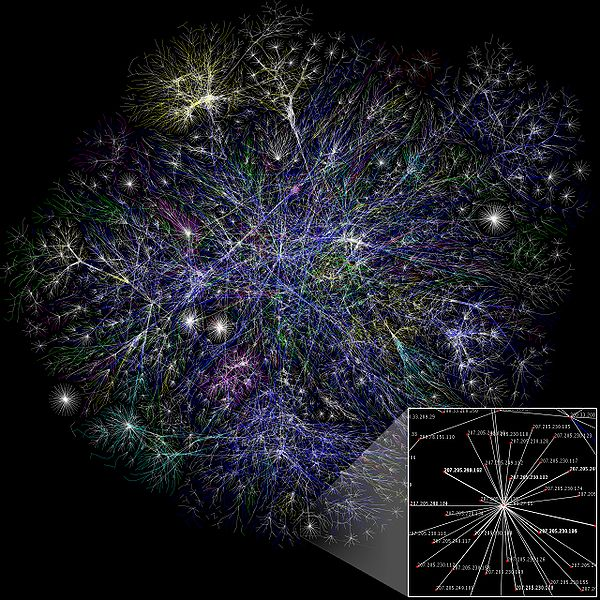
\includegraphics[scale=0.4]{backbone.jpg}
\end{center} 
\item WAN - Wide area network - mestá, štáty až medzikontinentálne. 
\item Internetwork - prepojenie viacerých sietí (napr. nackbone-om).
\end{itemize}
Niektoré sme vynechali. 

%%%%%%%%%%%%%%%%%%%%%%%%%%%%%%%%%%%%%%%
\subsection{Základné typy sietí, informačné toky}  
???
\begin{itemize}
\item Informačné 
\item Telekomunikačné
\item Sociálne
\item Neurónové, Náhodné,...            
\end{itemize}

%%%%%%%%%%%%%%%%%%%%%%%%%%%%%%%%%%%%%%%
\subsection{Zdroje, cieľové uzly, prepínací systém}
???
Asi niečo o sieťových zariadeniach. 
 
%%%%%%%%%%%%%%%%%%%%%%%%%%%%%%%%%%%%%%%
\subsection{Jednosmerné a obojsmerné spojenia}
       
\begin{itemize}                                  
\item Obojsmerné (full-duplex). Oboma smermi paralelne, ako mobilné telefóny.
\item Jednosmerné (half-duplex). Len jedným smerom naraz, ako policajné vysielačky.
\end{itemize} 
     
%%%%%%%%%%%%%%%%%%%%%%%%%%%%%%%%%%%%%%%
\subsection{Konferencie, komunikačné kanály}  
???
Dosť všeobecné. 
Konferenčné hovory boli implementované aj na telekomunikačných linkách. Jedným spôsobom boli špeciálne zariadenia - mosty - ktorým sa priradilo virtuálne telefónne číslo a na ňom sa zdielala komunikácia. Druhým spôsobom bolo (napr. v UK) pridanie špeciálneho tlačítka, ktoré umožňovalo zavolať tretiemu účastníkovy od druhého (predĺžiť tak spojenie $A \rightarrow B$ na $A \rightarrow B \rightarrow C$. 
  
%%%%%%%%%%%%%%%%%%%%%%%%%%%%%%%%%%%%%%%
\subsection{Multiplexovanie}   
\label{multiplexing}
Viacero komunikácií (protokolov, pagáčov makových) cez jednu linku. 
Napr. sťahovanie torrentov a pozeranie emailov naraz (resp. hranie age-a). 
Viac na \href{http://en.wikipedia.org/wiki/Multiplexing}{Wikipédií}.
       
%%%%%%%%%%%%%%%%%%%%%%%%%%%%%%%%%%%%%%%
\subsection{Virtuálne okruhy (virtual circuit)}     
Na sieťovej vrstve sa vytvorí cesta (obojsmerná) cez zariadenia, po ktorej sa posielajú dáta (bity, signály, fotóny, ...) medzi koncovými vrcholmi. Vytvorenie spojenia zaručuje, že dáta prídu v rovnakom poradí, ako boli odoslané. Opakom sú datagramy (napr. UDP), ktoré každý kus dát posielajú cez sieť (routre) neurčito.   
    
%%%%%%%%%%%%%%%%%%%%%%%%%%%%%%%%%%%%%%%%%%%%%%%%%%%%%%%%%%%%%%%%%%%%%%%%%%%%%%%%
\section{Schéma jednoduchého komunikačného modelu, sieťový software} 
???

%%%%%%%%%%%%%%%%%%%%%%%%%%%%%%%%%%%%%%%
\subsection{Technika štrukturovaného sieťového softwaru} 
???
  
%%%%%%%%%%%%%%%%%%%%%%%%%%%%%%%%%%%%%%%
\subsection{Koncepcia vrstiev, protokolov a interface} 
Pozri \ref{OSI}. 

%%%%%%%%%%%%%%%%%%%%%%%%%%%%%%%%%%%%%%%
\subsection{Virtuálna a fyzická komunikácia}      
???
Buď ju pozvem na večeru, alebo si chatujem na fejsbúčiku. 
                            
%%%%%%%%%%%%%%%%%%%%%%%%%%%%%%%%%%%%%%%%%%%%%%%%%%%%%%%%%%%%%%%%%%%%%%%%%%%%%%%%
\section{Všeobecné závery z oblasti počítačových sietí, ktoré musia byť zakomponované do vrstvovej sieťovej architektúry}   
%%%%%%%%%%%%%%%%%%%%%%%%%%%%%%%%%%%%%%%
\subsection{Adresovanie}    
Identifikovanie zariadení v rámci siete. Plochá addresácia (flat addressing) - adresy sa prideľujú inkrementovaním countera (alebo tomu izomorfným spôsobom), napr. MAC adresy.
Hierarchická adresácia (hierarchical addressing) - tvoria strom, napr. IP adresy (IANA prideľuje adresy kontinentom a štátom, tie prideľujú adresy ISP (Internet Service Provider, napr. Orange, T-com, ...),...) alebo telefónne čísla (keď ešte fungovali cez switche).
              
%%%%%%%%%%%%%%%%%%%%%%%%%%%%%%%%%%%%%%%
\subsection{Pravidlá pre prenos údajov}   
???
Prirovnáme to k cestnej doprave. 

%%%%%%%%%%%%%%%%%%%%%%%%%%%%%%%%%%%%%%%
\subsection{Správa chýb}
Integrita správ (checksumy), samoopravné kódy (\href{http://www.dcs.fmph.uniba.sk/texty/codebook.pdf}{Teória kódovania skriptá}). 
Robí sa to skoro na každej úrovni (hlavička aj telo (payload)).
                  
%%%%%%%%%%%%%%%%%%%%%%%%%%%%%%%%%%%%%%%
\subsection{Postupnosť (následnosť) správ}
V prípade point-to-point nie je čo riešiť. Ak sa dáta smerujú (routujú) cez viacero zariadení, tak nemusí byť zabezpečená, keďže môžu ísť rôznymi cestami (napr. keď sa router rozhodne predísť upchatiu na ďalšej linke). 
Ak je vytvorený virtuálny obvod, tak je postupnosť zabezpečená. Inak napr. TCP (\ref{TCP}).
 
%%%%%%%%%%%%%%%%%%%%%%%%%%%%%%%%%%%%%%%
\subsection{Problém rýchleho odosielateľa a pomalého príjemcu}
Pozri \href{http://en.wikipedia.org/wiki/Flow\_control}{Flow control}.
Rieši to napr. TCP pomocou posuvných okien (sliding windows, viac \ref{TCP}).
Problém je inštanciou problémov upchania siete (môže byť dôsledkom útoku),
presnejšie sa snaží upchaniu predchádzať (avoidance) ako riešiť vzniknuté (detection).
  
%%%%%%%%%%%%%%%%%%%%%%%%%%%%%%%%%%%%%%%
\subsection{Neschopnosť akceptovať správy ľubovoľnej dĺžky}  
Napr. $\infty$ dĺžky :)
Konkrétnym prípadom je získanie MTU (maximum transport unit) v IP paketoch. 
Nie všetky zariadenia vedia spracovať ľubovoľne dlhý paket. Napr. IPv4 umožňuje pakety sekať - \emph{fragmentácia paketov}, IPv6 definuje protokol na získanie MTU pre danú cestu a ponecháva na klientovi, aby zistil a dodržal túto hodnotu (inak bude jeho paket aj tak zahodený).

%%%%%%%%%%%%%%%%%%%%%%%%%%%%%%%%%%%%%%%
\subsection{Efektívny prenos malých správ} 
???
V dnešnej dobe, keď sa jeden klik klávesy pri SSH prenáša pomocou HTTP paketu?
(Asi 1000 násoboný overhead).
      
%%%%%%%%%%%%%%%%%%%%%%%%%%%%%%%%%%%%%%%
\subsection{Multiplexovanie a demultiplexovanie}  
Pozri \ref{multiplexing}. Demultiplexovanie je inverznou operáciou. 

%%%%%%%%%%%%%%%%%%%%%%%%%%%%%%%%%%%%%%%
\subsection{Smerovanie (routing)}     
Široká téma \href{http://en.wikipedia.org/wiki/Routing}{Routing}. 
Ide o to doručiť správy v prípade, že medzi komunikujúcimi zariadeniami neexistuje priame spojenie. 

\paragraph{Spôsoby doručenia.}
\begin{itemize}
\item Unicast - správa je určená jednému konkrétnemu.         
\item Broadcast - správa je určená všetkým v sieti (neposiela sa ďalej medzi siete - internetwork).
\item Multicat - správa sa posiela množine vrcholov. 
\item Anycast - správa sa doručuje práve jednému z množiny vrcholov (najčastejšie najbližšiemu).
\end{itemize}                               
                
\paragraph{Používané zariadenia.}
\begin{itemize}
\item Router. Pomocou \emph{routovacej tabuľky} $adresa_prijemcu \mapsto preposlat_na$ smeruje správy ďalej, resp. určenému príjemcovi.         
\item Bridge. Príjemcu hľadá pomocou floodingu - opýta sa každého v sieti (napr. protokol ARP \ref{ARP}, resp Neighbor Discovery v IPv6). Keď našiel, tak si ho zapamätá. Používa sa v malých sieťach, ako najnižší router.  
\item Gateway (nazývané aj protocol converters). Ich hlavným účelom je konverzia dát medzi dvoma protokolmi, resp. sú vstupnými bránami do iných \{$\epsilon$,pod,nad\}sietí. Využívajú sa na ľubovoľnej vrstve. 
\item Firewall. Preposiela, Zahadzuje (ničí) alebo Blokuje (pošle echo prečo) správy na základe jednoduchých pravidiel (port, protokol, IP adresa). Pracuje na sieťovej vrstve. Viac o firewalloch v \ref{firewall}. 
\item Switch. Narozdiel od hubu (kotrý preposiela správy všetkým ostatným), posiela správu len jej príjemcovi. 
\end{itemize}  

\paragraph{Routovacie tabuľky.} 
\begin{itemize}
\item Statické. Administrátor siete natvrdo zadá, kadiaľ sa majú preposielať dáta určené pre danú adresu.           
\item Adaptívne. Vo veľkých dynamických sieťach (napr. Internet) nie je možné konfigurovať staticky, preto si routre medzi sebou pravidelne vymieňajú informácie (každý router pozná zopár iných, napr. štandardný domáci router pozná router ISP). 
\end{itemize} 

Algoritmy na vypĺňanie routovaích tabuliek:
\begin{itemize}
\item Distance vector algorithms - Bellman-Ford ($O(n^3)$). Každej hrane sa priradí cena, potom zbehne algoritmus na výpočet vzdialeností (násobenie matice susednosti), správy od routra $R$ pre $A$ sa smerujú po najkratšej ceste. Tento prístup sa využíva v malých (lokálnych) sieťach. Môže sa použiť aj zložitejší Dijsktrou algoritmus, ale pre niektoré zariadenia môže byť príliš zložiťý.           
\item OLSR - Optimised Link State Routing - prehľadáva sa len do hĺbky 2, používa sa v ad-hoc sieťach (netreba vedieť). 
\item Path vector protocol - vytvorí sa hierarchická štruktúra, každý vrchol je zodpovedný za svojich priamych potomkov, použije sa hierarchická adresácia. Táto hierarchická štruktúra je updateovaná pomocou špecializovaných protokolov (\href{http://tools.ietf.org/html/rfc1322}{RFC-1322}). Používa s v medzisieťovom smerovaní.  
\end{itemize}
              
                                                         
%%%%%%%%%%%%%%%%%%%%%%%%%%%%%%%%%%%%%%%%%%%%%%%%%%%%%%%%%%%%%%%%%%%%%%%%%%%%%%%%
\section{Rozhrania a služby}                     
%%%%%%%%%%%%%%%%%%%%%%%%%%%%%%%%%%%%%%%
\subsection{Vzťah medzi vrstvami a rozhraniami}  
%%%%%%%%%%%%%%%%%%%%%%%%%%%%%%%%%%%%%%%
\subsection{Service Access Points (SAP's)}     
%%%%%%%%%%%%%%%%%%%%%%%%%%%%%%%%%%%%%%%
\subsection{Interface Data Unit}             
%%%%%%%%%%%%%%%%%%%%%%%%%%%%%%%%%%%%%%%
\subsection{Spojované a nespojované služby}  
%%%%%%%%%%%%%%%%%%%%%%%%%%%%%%%%%%%%%%%
\subsection{Kvalita služby a službové primitíva}            
%%%%%%%%%%%%%%%%%%%%%%%%%%%%%%%%%%%%%%%%%%%%%%%%%%%%%%%%%%%%%%%%%%%%%%%%%%%%%%%%
\section{Referenčné modely}           
%%%%%%%%%%%%%%%%%%%%%%%%%%%%%%%%%%%%%%%
\subsection{Ciele a nebezpečenstvá}   
%%%%%%%%%%%%%%%%%%%%%%%%%%%%%%%%%%%%%%%
\subsection{Open Systems Architecture} 
%%%%%%%%%%%%%%%%%%%%%%%%%%%%%%%%%%%%%%%
\subsection{Norma ISO 7498}                      
%%%%%%%%%%%%%%%%%%%%%%%%%%%%%%%%%%%%%%%%%%%%%%%%%%%%%%%%%%%%%%%%%%%%%%%%%%%%%%%%
\section{TCP/IP}    
\label{OSI}              
%%%%%%%%%%%%%%%%%%%%%%%%%%%%%%%%%%%%%%%
\subsection{Referenčný model}     
%%%%%%%%%%%%%%%%%%%%%%%%%%%%%%%%%%%%%%%
\subsection{Porovnanie a kritika OSI a TCP/IP referenčných modelov}    
OSI - Open systems interconnection. IP - Internet\footnote{Nie ten konkrétny} Protocol suite. Oba modely delia komunikáciu na abstraktné vrstvy. 
Každá vrstva má pdoobné funkcie a využíva funkcie susedných vrstiev. 

OSI:
\begin{itemize}
\item Aplikačná. Komunikácia medzi procesmi, majú špecializovanú úlohu (OSI definuje striktnejšie, IP zahŕňa aj Presentation a Session). DNS, FTP, HTTP, SMTP, DHCP. 
\item Prezentačná (občas nazývaná aj Syntax layer). Odbremeňuje koncové aplikácie od rôznych reprezentácií posielaných dát (znakových reťazcov),
napr. z dôvodu rôzneho kódovania koncových operačných systémov (ASCII, UTF, EBCDIC\footnote{
Extended Binary Coded Decimal Interchange Code (EBCDIC) is an 8-bit character encoding used mainly on IBM mainframe and IBM midrange computer operating systems.
}). Môže sa tu používať šifrovanie / dešifrovanie (aj keď nie nutne, napr. IPsec a VPN na sieťovej vrstve). SSL/TLS, MIME (Multipurpose Internet Mail Extensions).        
\item Session. Umožňuje koncovým aplikáciám (procesom) na koncových zariadeniach udržiavať stav spojenia (nie presne, pozri Session), napr. login na webstránkach. Využíva sa v RPC (Remote procedure calls - volanie procedúr koncových procesov) alebo pri streamovaní videa, aby zvuk nepredbiehal obraz a naopak. SOCKS, Named Pipe. 
\item Transportná. Sprístupnenie end-to-end komunikácie pre aplikácie, môže zabezpečovať spoľahlivosť, dátové prúdy a multiplexovanie. TCP, UDP.                    
\item Sieťová. Adresný priestor, smerovanie (routing) medzi koncovými stanicami. IP, ICMP, IPSec. 
\item Dátová. Vytváranie / posielanie základných logických jednotiek (postupnosti bitov) medzi fyzickými zariadeniami. Rámce (Frame), Switch, ATM (vytvára vituálne obvody)
\item Fyzická. Kabeláž. USB, Bluetooth, Wifi (IEEE 802.11).
\end{itemize}

Poznamenajme, že v skutočnosti je prvou hlavičkou hlavička fyzickej vrstvy. 

TCP/IP. Okrem vrstiev špecifikuje aj konkrétne protokoly. Internet tu neznamená konkrétny Internet, ale medzi-sieť.   
\begin{itemize}
\item Aplikačná. OSI + IMAP, POP, SOCKS, SSH.            
\item Transportná. Prenos dát medzi koncovými zariadeniami. Rovnaké ako OSI.     
\item Sieťová (Internet Layer). Adresácia a komunikácia medzi viacerými lokálnymi sieťami. IP (adresovanie), ICMP (reponse codes), IPsec.      
\item Linková. Kábeláž pre lokálne siete. MAC (6bytové adresy zariadení (sieťových kariet)). ARP (kto má MAC adresu s danou IP?), Ethernet, DSL, ISDN.      
\end{itemize}

Kritika: niečo pohaluzím. 
        
%%%%%%%%%%%%%%%%%%%%%%%%%%%%%%%%%%%%%%%%%%%%%%%%%%%%%%%%%%%%%%%%%%%%%%%%%%%%%%%%
\section{Teoretické základy pre dátovú komunikáciu} 
%%%%%%%%%%%%%%%%%%%%%%%%%%%%%%%%%%%%%%%
\subsection{Nyquistovo tvrdenie}               
%%%%%%%%%%%%%%%%%%%%%%%%%%%%%%%%%%%%%%%
\subsection{Shannonove odhady a ich dôsledky}  


%%%%%%%%%%%%%%%%%%%%%%%%%%%%%%%%%%%%%%%%%%%%%%%%%%%%%%%%%%%%%%%%%%%%%%%%%%%%%%%%
\section{Dátové prenosy}     
%%%%%%%%%%%%%%%%%%%%%%%%%%%%%%%%%%%%%%%
\subsection{UART}        
%%%%%%%%%%%%%%%%%%%%%%%%%%%%%%%%%%%%%%%
\subsection{USRT}     
%%%%%%%%%%%%%%%%%%%%%%%%%%%%%%%%%%%%%%%
\subsection{Synchronizácia}   


%%%%%%%%%%%%%%%%%%%%%%%%%%%%%%%%%%%%%%%%%%%%%%%%%%%%%%%%%%%%%%%%%%%%%%%%%%%%%%%%
\section{Elektromagnetické spektrum a bezdrôtové prenosy}  


%%%%%%%%%%%%%%%%%%%%%%%%%%%%%%%%%%%%%%%%%%%%%%%%%%%%%%%%%%%%%%%%%%%%%%%%%%%%%%%%
\section{Prenosové média a sieťové komponenty} 
%%%%%%%%%%%%%%%%%%%%%%%%%%%%%%%%%%%%%%%
\subsection{Techniky prepojovania sietí}  
%%%%%%%%%%%%%%%%%%%%%%%%%%%%%%%%%%%%%%%
\subsection{Charakter kabeláže}     
%%%%%%%%%%%%%%%%%%%%%%%%%%%%%%%%%%%%%%%
\subsection{Štruktúrovaná kabeláž}  
%%%%%%%%%%%%%%%%%%%%%%%%%%%%%%%%%%%%%%%
\subsection{Sieťové zariadenia}           

 
%%%%%%%%%%%%%%%%%%%%%%%%%%%%%%%%%%%%%%%%%%%%%%%%%%%%%%%%%%%%%%%%%%%%%%%%%%%%%%%%
\section{Linková vrstva}        
%%%%%%%%%%%%%%%%%%%%%%%%%%%%%%%%%%%%%%%
\subsection{MAC adresa (Media Access Control address)}     
Unikátny identifikátor pre sieťové zariadenia (sieťové karty napr.),
dodávané ich výrobcom. Má 6 byteov, prvé tri pre výrobcu (OUI - Organizationally Unique Identifier), ďalšie tri pre unikátny identifikátor (NIC - Network interface controller). Špeciálne $FF:FF:FF:FF:FF:FF$ je broadcastová adresa. 
          
MAC -  Media Access Control - akým spôsobom sa pristupuje k zdielanému médiu (na ktorom môže vysielať viacero staníc naraz).          
%%%%%%%%%%%%%%%%%%%%%%%%%%%%%%%%%%%%%%%
\subsection{IEEE štandardy 802 pre LAN (a WAN)}  
Február 1980. Rôzne veľkosti paketov. Rozdeľuje dátovú vrstvu na MAC  (predošlý odstavec) a LLC - Logical Link Control, ktorý umožňuje viacerým rôznym protokolom "paralelný" prístup k médiu (komunikačný kanál).

Je ich viacero, napr.:
\begin{itemize}
\item 802.3 Ethernet      
\item 802.11 Wireless LAN
\item 802.15.1 Bluetooth 
\end{itemize}

%%%%%%%%%%%%%%%%%%%%%%%%%%%%%%%%%%%%%%%
\subsection{FDDI (Fiber Distributed Data Interface)}  
Sieťová karta. Umožňuje prenos 100Mbit/s, na kružnicovej topológií (zdielané médium). Používal sa v LAN. Nahradený Fast Ethernet.    
                 
%%%%%%%%%%%%%%%%%%%%%%%%%%%%%%%%%%%%%%%
\subsection{Fast Ethernet}            
Lacný, všade používaný (nazývaný aj LAN kábel).
100Mbit / s. Hviezdicová topológia (centrom je Hub, Switch alebo Router).
Používa CSMA/CD (Detekcia kolízií s náhodným čakaním (podľa exponenciálnej distribúcie pravdepodobnosti = \emph{exponential backoff}) v prípade kolízie). Viacero verzií podľa druhu vodiča (medené / optické).

%%%%%%%%%%%%%%%%%%%%%%%%%%%%%%%%%%%%%%%
\subsection{Gigabit Ethernet}       
Od roku 2010 "common and economical" (štandardizované 1998). Pomocou switchov je umožnená full-duplex komunikácia (obojsmerná). 
Zas asi 10 verzií (od 25m po 70 km), (asi vždy) optické vlákna. 

%%%%%%%%%%%%%%%%%%%%%%%%%%%%%%%%%%%%%%%
\subsection{10 Gigabit Ethernet}  
Len full-duplex (obojsmerne), nedá sa použiť s hubmi ani s CSMA/CD. 
Od roku 2002. Problémom sú 10Gbit routre (podľa istých zdrojov realizovateľné na moderných grafickách kartách, lepšie ako bitcoiny). Optické káble. Zas kopa verzií, typovo rovnakých. 

%%%%%%%%%%%%%%%%%%%%%%%%%%%%%%%%%%%%%%%
\subsection{802.11 (Wireless LAN)}  

Pozri \href{http://netlab.dcs.fmph.uniba.sk/siete/cviko2/}{Cviká z počítačových sietí}, ďalej len výcuc. 
CSMA (Carrier Sense Multiple Access - Collision avoidance) - ak je linka obsadená, tak exponential backoff. Zdielané médium - 2.4GHz až 5GHz pásma. 
Antény ovplyvňujú kvalitu. Viacero protokolov (rôzne prenosové rýchlosti).

Stanica (Station) je zariadením vo WiFi sieti. BSS (Basic Service Set) - zariadenia, ktoré vedia medzi sebou komunikovať v dvoch režimoch:
\begin{itemize}
\item \emph{Ad-hoc} režim, alebo tiež IBSS (Independent Basic Service Set) sa používa v prípade, keď je treba jednoduchým spôsobom vytvoriť bezdrôtovú sieť. Prvá stanica vytvárajúca sieť náhodne zvolí BSSID, začne vysielať majáčiky (beacons) oznamujúce prítomnosť siete a ostatné stanice komunikujú priamo medzi sebou. Ak stanice dlhšiu dobu nedostanú beacon, predpokladajú, že prvá stanica vypadla a zvyšné stanice v náhodnom čase začnú vysielať beacony (prvá stanica vyhráva).
\item \emph{Infrastructure} režim obsahuje stanicu, ktorá zároveň plní úlohu prístupového bodu -- AP (Access Point), s ktorou komunikujú všetky ostatné stanice (dve stanice môžu vždy komunikovať iba cez AP).
\end{itemize}
     
Problém s bezpečnosťou (ľahké zachytávania paketov). Zabezpečenie: 
\begin{itemize}                                                 
\item Bez šifrovania -- najstarší, najjednoduchší, najnebezpečnejší.
\item WEP (Wired Equivalent Privacy). Šifra RC4 (64-128bitový)        
\item WPA (Wi-Fi Protected Access). Namiesto RC4 TKIP (Temporal Key Interchange Protocol) - časté menenie kľúčov (neprichádza k celkovému odhaleniu komunikácie pri odhlení jedného kľúča).
\item WPA2. Novšia verzia. 
\item EAP (použivaný aj v point-to-point). Má oveľa širšie možnosti autentifikácie (meno/heslo, certifikát, ...).
\end{itemize}
      
Distribučný systém - prepojenie viacerých WiFi routrov (staníc) medzi sebou Ethernetom alebo bezdrátovo. Treba myslieť na MAC adresy, keďže nemusia byť pod daným routrom. 

Mesh networking (také peer-to-peer). Každý je rovnocenný, preposiela pakety ďalej (chová sa ako wifi router). Nie je rozšírené. 
      
%%%%%%%%%%%%%%%%%%%%%%%%%%%%%%%%%%%%%%%
\subsection{802.15 (Wireless PAN)} 
PAN - personal area network - len medzi zariadenia používané jednou osobou (napr.:mobil, tablet, notebook, desktop, mp3 player) - nazýva sa aj \emph{Body Area Network}.
Bluetooth, WiFi (staré infraporty a ďalšie). 
%%%%%%%%%%%%%%%%%%%%%%%%%%%%%%%%%%%%%%%
\subsection{802.16 (Wireless broadband)}
Ako mobilná sieť, ale ponúka bezdrátové pripojenie k Internetu.
Viac na \href{http://en.wikipedia.org/wiki/Broadband\_Wireless\_Access}{Broadband Wireless Access}. 
       
%%%%%%%%%%%%%%%%%%%%%%%%%%%%%%%%%%%%%%%
\subsection{Bluetooth}           
Výmena dát na krátku vzdialenosť. Každý pozná. 
Dosť komplikovaná implementácia. 
                                                 
%%%%%%%%%%%%%%%%%%%%%%%%%%%%%%%%%%%%%%%%%%%%%%%%%%%%%%%%%%%%%%%%%%%%%%%%%%%%%%%%
\section{Sieťová vrstva}                      
%%%%%%%%%%%%%%%%%%%%%%%%%%%%%%%%%%%%%%%
\subsection{Interná organizácia sieťovej vrstvy} 
%%%%%%%%%%%%%%%%%%%%%%%%%%%%%%%%%%%%%%%
\subsection{Príklad prenosu packetov cez sieť} 
%%%%%%%%%%%%%%%%%%%%%%%%%%%%%%%%%%%%%%%
\subsection{Uzly a smerovacie tabuľky}     
%%%%%%%%%%%%%%%%%%%%%%%%%%%%%%%%%%%%%%%
\subsection{IP protokol}               
%%%%%%%%%%%%%%%%%%%%%%%%%%%%%%%%%%%%%%%
\subsection{Smerovanie}             
%%%%%%%%%%%%%%%%%%%%%%%%%%%%%%%%%%%%%%%
\subsection{CIDR, tunelovanie}                                                                     
%%%%%%%%%%%%%%%%%%%%%%%%%%%%%%%%%%%%%%%%%%%%%%%%%%%%%%%%%%%%%%%%%%%%%%%%%%%%%%%%
\section{Transportná vrstva}        
%%%%%%%%%%%%%%%%%%%%%%%%%%%%%%%%%%%%%%%
\subsection{Protokoly TCP a UDP}   
%%%%%%%%%%%%%%%%%%%%%%%%%%%%%%%%%%%%%%%
\subsection{Vytváranie, riadenie a ukončovanie spojenia v TCP} 
%%%%%%%%%%%%%%%%%%%%%%%%%%%%%%%%%%%%%%%
\subsection{SSL}                             
%%%%%%%%%%%%%%%%%%%%%%%%%%%%%%%%%%%%%%%%%%%%%%%%%%%%%%%%%%%%%%%%%%%%%%%%%%%%%%%%
\section{Aplikačná vrstva a podporné protokoly}            
%%%%%%%%%%%%%%%%%%%%%%%%%%%%%%%%%%%%%%%%%%%%%%%%%%%%%%%%%%%%%%%%%%%%%%%%%%%%%%%%
\section{Telefónny systém}    
%%%%%%%%%%%%%%%%%%%%%%%%%%%%%%%%%%%%%%%
\subsection{Modemy}      
%%%%%%%%%%%%%%%%%%%%%%%%%%%%%%%%%%%%%%%
\subsection{Štandardy}    
%%%%%%%%%%%%%%%%%%%%%%%%%%%%%%%%%%%%%%%
\subsection{Konštelačné vzorky}  
%%%%%%%%%%%%%%%%%%%%%%%%%%%%%%%%%%%%%%%
\subsection{Modulačné techniky}   
%%%%%%%%%%%%%%%%%%%%%%%%%%%%%%%%%%%%%%%
\subsection{ISDN - systém pre domáce a firemné využitie}  
%%%%%%%%%%%%%%%%%%%%%%%%%%%%%%%%%%%%%%%
\subsection{xDSL, B-ISDN}       
%%%%%%%%%%%%%%%%%%%%%%%%%%%%%%%%%%%%%%%%%%%%%%%%%%%%%%%%%%%%%%%%%%%%%%%%%%%%%%%%
\section{Diaľkové vedenia a multiplexovanie, optické siete}
%%%%%%%%%%%%%%%%%%%%%%%%%%%%%%%%%%%%%%%
\subsection{FDMA/TDMA/CDMA}                           
%%%%%%%%%%%%%%%%%%%%%%%%%%%%%%%%%%%%%%%
\subsection{Synchrónne optické siete (SDH, SONET architektúra - definícia rámcov v SDH)}



\section{Referencie a odporúčaná literatúra}
\begin{itemize}                                
\item \url{http://en.wikipedia.org} 
\item \url{http://netlab.dcs.fmph.uniba.sk/siete/} 
\item \url{http://www.dcs.fmph.uniba.sk/\~plachetk/TEACHING/DISTRSYS2012/siete.pdf} 
\end{itemize}

\section{Ďalšie pojmy}
\begin{itemize}
\item lip synch (VoIP)                                  
\item \emph{ATM} is a core protocol used over the SONET/SDH backbone of the public switched telephone network (PSTN) and Integrated Services Digital Network (ISDN), but its use is declining in favour of All IP. 
\end{itemize}

\end{document}
